\documentclass[11pt,a4paper]{article}
\usepackage{graphicx}
\usepackage{listings}
\usepackage{xcolor}
\usepackage{polski}
\usepackage{amsmath}
\usepackage[utf8]{inputenc}
\usepackage{rotating}
\usepackage{tabularx}
\usepackage{float}
\usepackage{url}
\usepackage{array}
\newcolumntype{L}[1]{>{\raggedright\let\newline\\\arraybackslash\hspace{0pt}}m{#1}}
\newcolumntype{C}[1]{>{\centering\let\newline\\\arraybackslash\hspace{0pt}}m{#1}}
\newcolumntype{R}[1]{>{\raggedleft\let\newline\\\arraybackslash\hspace{0pt}}m{#1}}

\begin{document}
\begin{titlepage}
\begin{center}

\textsc{\Huge KATEDRA INFORMATYKI}\\[1.0cm]
\textsc{\LARGE Wydział Informatyki, Elektorniki i Telekomunikacji AGH}\\[1.0cm]

\includegraphics[width=0.4\textwidth]{../images/logo}~\\[1cm]

{ \Huge \bfseries Badania Operacyjne}\\[0.5cm]
\textsc{\Large Optymalizacja trasy w trybie online}\\[1.0cm]

\emph Krzysztof \textsc{Trzepla} \\

\vfill
{\large \today}

\end{center}
\end{titlepage}


\tableofcontents
\newpage

\section{Wstęp}

Niniejszy projekt ma na celu zbadanie wpływu dynamicznych zmian trasy pojazdu, w zależności od panujących warunków, na sumaryczny czas przejazdu. W pierwszej części opracowania przedstawiony zostanie sposób modelowania ruchu drogowego z wykorzystaniem symulatora \emph{SUMO} oraz wykorzystane w modelowaniu narzędzia, m.in. biblioteka \emph{TraCI}. W drugiej części opracowania opisana zostanie utworzona aplikacja oraz proces symulacji. W trzeciej części znajdzie się opis przeprowadzonych testów wraz z danymi w formie wykresów oraz tabel. W czwartej, ostatniej części opracowania dokonana zostanie analiza otrzymanych wyników wraz z podsumowaniem oraz wnioskami.

Kod źródłowy projektu znajduje się na płycie CD załączonej do dokumentacji. Dodatkowo znajduje się w repozytorium pod adresem: \url{https://github.com/OR2013/OnlinePathOptimalization}.

\section{Modelowanie ruchu drogowego}

Istnieje wiele narzędzi umożliwiających symulację ruchu drogowego. W niniejszym projekcie wykorzystano symulator \emph{SUMO} utworzony przez pracowników \emph{Instytutu Transportu Niemieckiej Agencji Kosmicznej} i udostępniony na licencji \emph{GPL}.

\subsection{Symulator SUMO}

\emph{\textbf{S}imulation of \textbf{U}rban \textbf{MO}bility}, w skrócie \emph{SUMO}, to wysoce wyspecjalizowany symulator umożliwiający wytworzenie sieci połączeń oraz badanie zachowania pojazdów w ruchu drogowym.\\[0.2cm]

Cechy symulatora:
\begin{itemize}
	\item możliwość wygenerowania sieci połączeń oraz ruchu drogowego bez konieczności korzystania z innych aplikacji
	\item ciągły w czasie i przestrzeni ruch pojazdów
	\item ruch każdego pojazdu jest modelowany oddzielnie
	\item duży wybór dostępnych pojazdów (samochody osobowe, samochody ciężarowe, autobusy, itp.)
	\item duży wybór dostępnych dróg (jednopasmowe, wielopasmowe)
	\item możliwość wprowadzenia oraz sterowania sygnalizacją świetlną
	\item możliwość komunikacji z zewnętrznymi aplikacjami, m.in. biblioteka \emph{TraCi}
	\item konfiguracja symulatora, opis sieci oraz ruchu drogowego z wykorzystaniem plików XML
\end{itemize} 

\subsection{Biblioteka TraCI}

\emph{\textbf{Tra}ffic \textbf{C}ontrol \textbf{I}nterface}, w skrócie \emph{TraCI}, to biblioteka pozwalająca na dynamiczne pobieranie danych na temat obiektów będących częścią symulacji oraz modyfikowanie ich zachowania w danym kroku symulacji. Komunikacja z procesem symulującym ruch drogowy odbywa się z wykorzystaniem socketu TCP. Domyślny numer portu na którym nasłuchuje proces symulujący wynosi 8813. Pełna dokumentacja biblioteki znajduje się pod adresem \url{http://sumo-sim.org/pydoc/traci.html}.

\subsection{Aplikacja Netgenerate}

\emph{Netgenerate} to aplikacja, będąca częścią projektu \emph{SUMO}, umożliwiająca wygenerowanie sieci drogowej, która następnie jest wykorzystywana przez symulator. Szeroka gama parametrów obsługiwanych przez aplikację pozwala na generację różnorodnych sieci drogowych.\\[0.5cm]
W projekcie wkorzystano następujące opcje aplikacji \emph{Netgenerate}:
\begin{description}
	\item[--random] - tworzenie sieci drogowej o losowej strukturze
	\item[--rand.iterations] - ilość krawędzi (ulic) w sieci drogowej
	\item[--rand.max-distance] - maksymalna długość krawędzi (ulicy) w sieci drogowej
	\item[--no-turnarounds] - zakaz zawracania na skrzyżowaniach
	\item[--output] - plik w formacie XML stanowiący opis sieci drogowej
\end{description}

\subsection{Skrypt randomTrips}

Skrypt \emph{randomTrips} umożliwia wytworzenie punktów startowych i docelowych dla poszczególnych pojazdów, a następnie znalezienie trasy łączącej zaproponowane punkty. Powstały ruch drogowy jest zapisywany w formacie XML odpowiednim dla symulatora \emph{SUMO}.\\[0.5cm]
W projekcie wykorzystano następujące opcje skryptu \emph{randomTrips}:
\begin{description}
	\item[-e] - okres trwania ruchu drogowego
	\item[-p] - częstotliwość określająca pojawianie się nowych samochodów w sieci drogowej
	\item[--fringe-factor] - prawdopodobieństwo, że trasa poszczególnych pojazdów będzie się rozpoczynać i kończyć na obrzeżach sieci drogowej
	\item[-n] - plik zawierający opis sieci drogowej w formacie XML (wygenerowany przez aplikację \emph{Netgenerate})
	\item[-r] - plik w formacie XML stanowiący opis ruchu drogowego 
\end{description}

\section{Aplikacja}

\subsection{Opis}

W ramach projektu utworzona została aplikacja umożliwiająca badanie wpływu dynamicznych zmian trasy wybranego pojazdu na sumaryczny czas podróży. 

\subsubsection{Struktura aplikacji}

Centralny punkt aplikacji stanowi moduł symulacyjny. Jest on odpowiedzialny za wygenerowanie sieci i ruchu drogowego oraz za przeprowadzenie symulacji (zainicjowanie symulatora, komunikację z symulatorem). Diagram klas modułu symulacyjnego zamieszczony jest poniżej:

\begin{figure}[H]
	\centering
		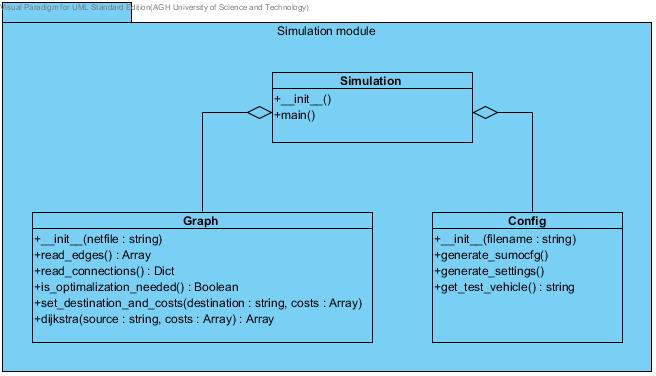
\includegraphics[width=\textwidth]{../images/class_diagram}
	\caption{Diagram klas.}
\end{figure}

W projekcie wyróżniamy następujące komponenty:
\begin{itemize}
	\item moduł symulacyjny
	\item symulator \emph{SUMO}
	\item biblioteka \emph{TraCI}
	\item aplikacja \emph{Netgenerate}
	\item skrypt \emph{randomTrips}
\end{itemize}

\begin{figure}[H]
	\centering
		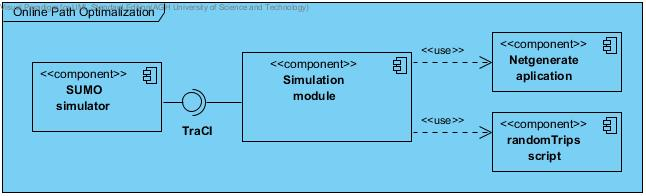
\includegraphics[width=\textwidth]{../images/component_diagram}
	\caption{Diagram komponentów.}
\end{figure}


\subsubsection{Proces symulacji}

Symulacja przebiega w następujących krokach:

\begin{enumerate}
	\item Wygenerowanie sieci drogowej przy pomocy aplikacji \emph{Netgenerate}.
	\item Wygenerowanie ruchu drogowego przy pomocy skryptu \emph{randomTrips}.
	\item Uruchomienie symulacja w której podejmuje się próbę optymalizacji trasy wybranego pojazdu (pojawiającego się mniej więcej w połowie czasu trwania symulacji, tak aby w sieci drogowej istniał ruch) na podstawie aktualnego stanu dróg (oczekiwanego czasu przejazdu).
	\item Poszukiwanie szybszej trasy dojazdu jest inicjowane gdy spełnione są następujące warunki:
	\begin{itemize}
		\item pojazd, którego trasa jest optymalizowana, pokonał co najmniej 0.9 odcinka obecnej drogi
		\item nastąpiło wydłużenie czasu przejazdu przez któryś z odcinków należących do aktualnej trasy samochodu lub nastąpiło skrócenie czasu przejazdu przez któryś z odcinków nie należących do aktualnej trasy samochodu. W obu przypadkach rozpatrywane są tylko zmiany, których różnica względem początkowego stanu dróg jest większa od parametru \textit{alpha}.
	\end{itemize}
	\item Ponowienie symulacji przejazdu wybranego pojazdu dla takiego samego stanu dróg oraz ruchu drogowego, z tą różnicą że tym razem trasa nie jest optymalizowana online, a pojazd porusza się z góry ustaloną (najlepszą w chwili początkowej) trasą. 
\end{enumerate}

\subsubsection{Parametry aplikacji}

Aplikacja udostępnia następujące parametry:
\begin{description}
	\item[--nogui] - symulacja bez wizualizacji
	\item[--nogen] - symulacja bez generowania sieci oraz ruchu drogowego
	\item[--prefix] - prefiks nazw tworzonych plików XML
	\item[--size] - rozmiar sieci drogowej
	\item[--alpha] - parametr określający jak duże zmiany czasu przejazdu są uwzględniane
	\item[--rate] - częstotliwość z jaką pojawiają się pojazdy w sieci
	\item[--verbose] - szczegółowe informacje na temat symulacji
	\item[--max-distance] - maksymalna długość krawędzi (ulicy) w generowanej sieci drogowej
\end{description}

\subsubsection{Makefile}

Do aplikacji dołączony jest plik \textit{Makefile} automatyzujący procesy testowania aplikacji, przeprowadzania eksperymentów oraz generowania dokumentacji.\\[0.5cm]
\textit{Makefile} udostępnia następujące parametry:
\begin{description}
	\item[make test] - uruchomienie załączonych testów aplikacji
	\item[make simulations] - przeprowadzenie wszystkich zdefiniowanych eksperymentów
	\item[make simulation(nr)] - przeprowadzenie eksperymentu numer \textit{nr}, gdzie $1 <= nr <= 7$
	\item[make graphs] - wygenerowanie wykresów
	\item[make docs] - wygenerowanie dokumentacji projektu
\end{description}

\subsubsection{Testy}

W celu sprawdzenia poprawności funkcji udostępnianych przez aplikacje do projektu załączono testy jednostkowe. Można je uruchomić wydając w katalogu głównym projektu polecenie \textit{make test}. 

Testy jednostkowe:
\begin{description}
	\item[test read edges] - test sprawdzający poprawność wczytania struktury sieci drogowej
	\item[test read connections] - test sprawdzający poprawność wczytania połączeń w sieci drogowej
	\item[test is optimalization needed] - test sprawdzający poprawność warunków w których następuje optymalizacja trasy
	\item[test dijkstra simple] - test sprawdzający poprawność implementacji algorytmu Dijkstry dla grafu o dziesięciu wierzchołkach
	\item[test dijkstra complex] - test sprawdzający poprawność implementacji algorytmu Dijkstry dla grafu o tysiącu wierzchołków
\end{description}

\subsection{Algorytm Dijkstry}

W projekcie poszukiwanie szybszej trasy dojazdu odbywa się z wykorzystaniem algorytmu Dijkstry.

\subsubsection{Opis}

Przez $s$ oznaczamy wierzchołek źródłowy, $w(i, j)$ to waga krawędzi $(i, j)$ w grafie.

\begin{itemize}
	\item Stwórz tablicę $d$ odległości od źródła dla wszystkich wierzchołków grafu. Na początku $d[s]=0$, zaś $d[v]=\infty$ dla wszystkich pozostałych wierzchołków.
	\item Utwórz kolejkę priorytetową $Q$ wszystkich wierzchołków grafu. Priorytetem kolejki jest aktualnie wyliczona odległość od wierzchołka źródłowego $s$.
	\item Dopóki kolejka nie jest pusta:
	\begin{itemize}
		\item Usuń z kolejki wierzchołek $u$ o najniższym priorytecie (wierzchołek najbliższy źródła, który nie został jeszcze rozważony)
		\item Dla każdego sąsiada $v$ wierzchołka $u$ dokonaj \textit{relaksacji} poprzez $u$: jeśli $d[u] + w(u, v) < d[v]$ (poprzez $u$ da się dojść do $v$ szybciej niż dotychczasową ścieżką), to $d[v] := d[u] + w(u, v)$.
	\end{itemize}
	\item Na końcu tablica $d$ zawiera najkrótsze odległości do wszystkich wierzchołków.
\end{itemize}

Dodatkowo możemy w tablicy \textit{poprzednik} przechowywać dla każdego wierzchołka numer jego bezpośredniego poprzednika na najkrótszej ścieżce, co pozwoli na odtworzenie pełnej ścieżki od źródła do każdego wierzchołka - przy każdej relaksacji w ostatnim punkcie $u$ staje się poprzednikiem $v$.

\section{Symulacje}

W celu zbadanie wpływu dynamicznych zmian trasy wybranego pojazdu na sumaryczny czas podróży przeprowadzono szereg symulacji, których specyfikacja znajduje się poniżej. Zamieszczone wyniki są wartościami średnimi pochodzącymi z dziesięciu prób.

\subsection{Symulacja 1}

\subsubsection{Opis}

Pierwsza symulacja miała na celu sprawdzenie jak optymalizacja trasy w trybie online oddziałuje na czas podróży dla różnych wielkości sieci drogowych. Parametr \textit{alpha} wynosił \emph{0.05}, częstotliwość pojawiania się samochodów w sieci drogowej wynosiła \emph{2 kroki symulacji/pojazd} oraz maksymalna długość ulicy wynosiła \emph{500 metrów}.

\subsubsection{Wyniki}

\begin{table}[H]
\begin{tabular}{ | C{4cm} | C{4cm} | C{4cm} | }
\hline
Rozmiar sieci drogowej [ulica] & Optymalizacja [krok symulacji] & Brak optymalizacji [krok symulacji] \\ \hline
10 & 123.8 & 121.6 \\ \hline
20 & 137.8 & 143.7 \\ \hline
30 & 122.5 & 122.1 \\ \hline
40 & 173.5 & 171.4 \\ \hline
50 & 213.2 & 216.4 \\ \hline
60 & 213.9 & 230.2 \\ \hline
70 & 174.8 & 178.2 \\ \hline
80 & 214.1 & 215.7 \\ \hline
90 & 250.4 & 258.3 \\ \hline
100 & 219.4 & 219.8 \\ \hline
200 & 355.2 & 368 \\ \hline
300 & 373.7 & 379.8 \\ \hline
400 & 411.1 & 423.3 \\ \hline
500 & 493.6 & 501.6 \\ \hline
600 & 465.3 & 475.7 \\ \hline
700 & 420 & 422.3 \\ \hline
800 & 599.7 & 606.2 \\ \hline
900 & 659.3 & 666 \\ \hline
1000 & 581 & 581.3 \\ \hline
\hline
\end{tabular}
\caption{Zależność czasu przejazdu od rozmiaru sieci drogowej.}
\end{table}


\begin{figure}[H]
	\centering
		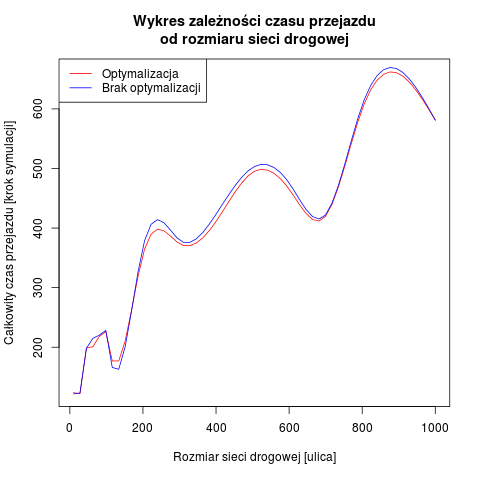
\includegraphics[width=0.7\textwidth]{../images/simulation1}
	\caption{Zależność czasu przejazdu od rozmiaru sieci drogowej.}
\end{figure}

\begin{figure}[H]
	\centering
		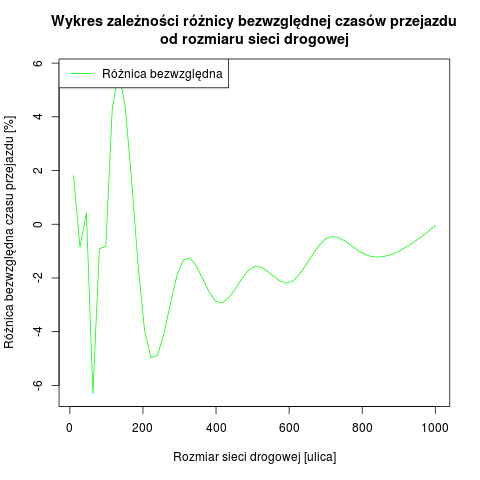
\includegraphics[width=0.7\textwidth]{../images/simulation1_diff}
	\caption{Zależność bezwzględnej różnicy czasów przejazdu od rozmiaru sieci drogowej.}
\end{figure}

\subsubsection{Analiza wyników}

Analiza otrzymanych wyników pozwala stwierdzić korzystny wpływ zastosowanej metody optymalizacyjnej na sumaryczny czas przejazdu. W znakomitej większości przypadków czas przejazdu pojazdu, którego trasa była zmienia dynamicznie w zależności od sytuacji panującej w sieci drogowej, okazał się być krótszy od czasu przejazdu dla pojazdu poruszającego się niezmienną trasą. Przewaga wspomnianej metody jest szczególnie widoczna dla średnich grafów o rozmiarze wahającym się od dwustu do trzystu krawędzi i wynosi około 5 procent. Jest to związane z ilością możliwych ścieżek od punktu początkowego do końcowego. Dla małych grafów ilość możliwych ścieżek łączących dwa zadane wierzchołki jest niewielka, a co za tym idzie możliwości wybrania lepszej trasy dojazdu są ograniczone. Z kolei dla dużych grafów liczba ta jest dużo większa, stąd ryzyko podejmowania decyzji nieoptymalnych w skali globalnej jest bardziej prawdopodobne. 

\subsection{Symulacja 2}

\subsubsection{Opis}

Druga symulacja polegała na zbadaniu wpływu parametru \textit{alpha} na sumaryczny czas podróży. Rozmiar sieci drogowej wynosił \textit{100 ulic}, częstotliwość pojawiania się samochodów w sieci drogowej wynosiła \emph{2 kroki symulacji/pojazd} oraz maksymalna długość ulicy wynosiła \emph{500 metrów}.

\subsubsection{Wyniki}

\begin{table}[H]
\begin{tabular}{ | C{4cm} | C{4cm} | C{4cm} | }
\hline
Parametr alpha [j] & Optymalizacja [krok symulacji] & Brak optymalizacji [krok symulacji] \\ \hline
0.01 & 250.4 & 257.7 \\ \hline
0.02 & 247.3 & 256.2 \\ \hline
0.05 & 218.3 & 222.3 \\ \hline
0.1 & 231.7 & 234.8 \\ \hline
0.2 & 232.3 & 233.3 \\ \hline
0.5 & 230.1 & 238.5 \\ \hline
1 & 203.4 & 212 \\ \hline
2 & 166.9 & 167.3 \\ \hline
5 & 267 & 270.5 \\ \hline
10 & 255.1 & 258.5 \\ \hline
\hline
\end{tabular}
\caption{Zależność czasu przejazdu od parametru \textit{alpha}'.}
\end{table}


\begin{figure}[H]
	\centering
		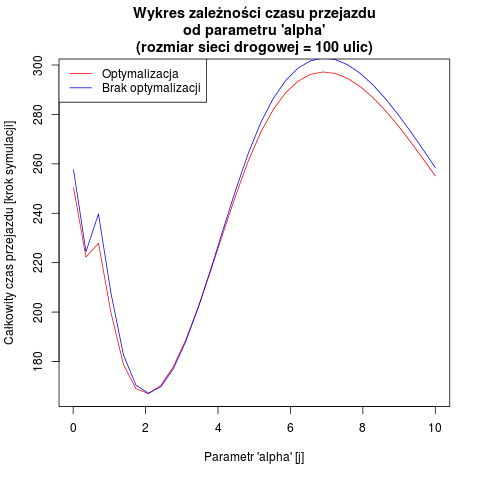
\includegraphics[width=0.7\textwidth]{../images/simulation2}
	\caption{Zależność czasu przejazdu od parametru \textit{alpha}.}
\end{figure}

\begin{figure}[H]
	\centering
		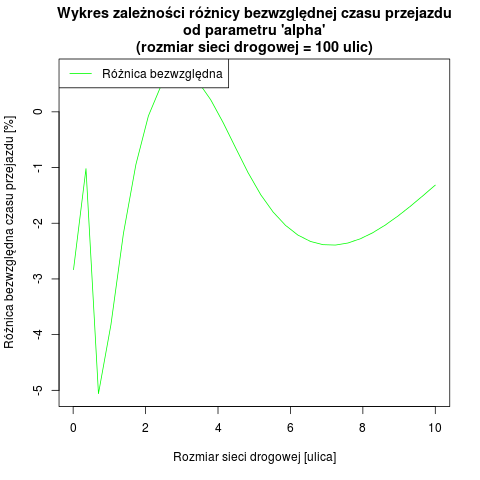
\includegraphics[width=0.7\textwidth]{../images/simulation2_diff}
	\caption{Zależność bezwzględnej różnicy czasów przejazdu od parametru \textit{alpha}.}
\end{figure}

\subsubsection{Analiza wyników}

Parametr \textit{alpha} określał czy zmiana czasu przejazdu przez daną krawędź jest istotna z punktu widzenia metody optymalizacyjnej. Uzyskane wyniki pozwalają stwierdzić, że dla grafów rozmiaru około stu krawędzi średnie czasy przejazdu są najlepsze dla wartości parametru \textit{alpha} wynoszącej około 3 do 4. Oznacza to, że najkorzystniejsze okazało się uwzględnianie zmian, które trzy do czterokrotnie wydłużały czas przejazdu przez daną krawędź. Wynika to z faktu, że analizowanie niewielkich zmian czasu przejazdu może prowadzić do podejmowania częstych i prawdopodobnie nieoptymalnych decyzji zmian trasy. Natomiast dla dużych wartości parametru \textit{aplha} znakomita większość zmian jest odrzucana, a co za tym idzie nie jest dokonywana optymalizacja trasy przejazdu.

\subsection{Symulacja 3}

\subsubsection{Opis}

Trzecia symulacja była powtórzeniem symulacji drugiej, z tą różnica, że rozmiar sieci drogowej wynosił \textit{1000 ulic}.

\subsubsection{Wyniki}

\begin{table}[H]
\begin{tabular}{ | C{4cm} | C{4cm} | C{4cm} | }
\hline
Parametr alpha [j] & Optymalizacja [krok symulacji] & Brak optymalizacji [krok symulacji] \\ \hline
0.01 & 505.1 & 518.2 \\ \hline
0.02 & 503.1 & 502.6 \\ \hline
0.05 & 448.888888888889 & 455.444444444444 \\ \hline
0.1 & 489.9 & 490.8 \\ \hline
0.2 & 522.1 & 523.8 \\ \hline
0.5 & 489.8 & 493.6 \\ \hline
1 & 546.1 & 552.6 \\ \hline
2 & 439.9 & 457.6 \\ \hline
5 & 513.4 & 531.6 \\ \hline
10 & 578.9 & 585.7 \\ \hline
\hline
\end{tabular}
\caption{Zależność czasu przejazdu od parametru \textit{alpha}'.}
\end{table}


\begin{figure}[H]
	\centering
		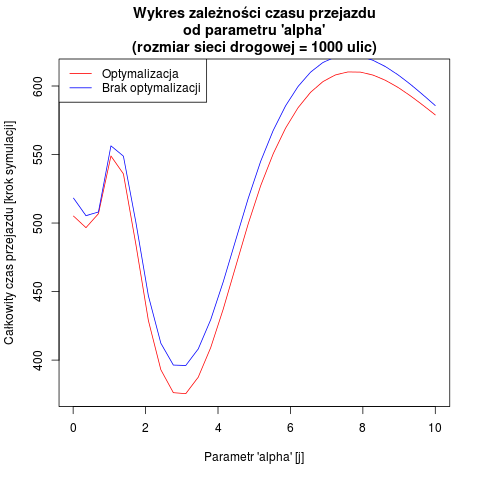
\includegraphics[width=0.7\textwidth]{../images/simulation3}
	\caption{Zależność czasu przejazdu od parametru \textit{alpha}.}
\end{figure}

\begin{figure}[H]
	\centering
		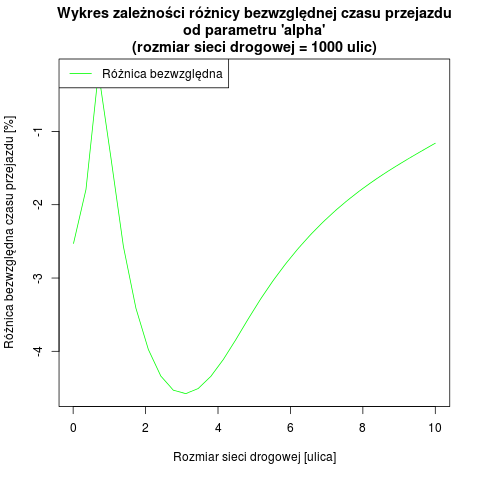
\includegraphics[width=0.7\textwidth]{../images/simulation3_diff}
	\caption{Zależność bezwzględnej różnicy czasów przejazdu od parametru \textit{alpha}.}
\end{figure}

\subsubsection{Analiza wyników}

Symulacja trzecia podobnie jak symulacja druga sprawdzała wpływ parametru \textit{alpha} na sumaryczny czas podróży. Tym razem okazało się jednak, że najkorzystniejsze wyniki (poprawa czasu przejazdu rzędu 5 procent) są uzyskiwane dla parametru \textit{alpha} wynoszącego od 2 do 3. Pozwala to stwierdzić, że wraz ze wzrostem rozmiaru sieci drogowej należy uwzględniać mniejsze zmiany czasu przejazdu przez krawędzie. Wynika to z kształtowania się ruchu drogowego. Im większa sieć drogowa tym mniejsze prawdopodobieństwo powstawania zatorów i oczekiwania na skrzyżowaniach.

\subsection{Symulacja 4}

\subsubsection{Opis}

Czwarta symulacja badała zależność czasu przejazdu od częstotliwości pojawiania się samochodów w sieci drogowej, a co za tym idzie od natężenia ruchu. Rozmiar sieci drogowej wynosi \textit{100 ulic}, parametr \textit{alpha 0.05}, a maksymalna długość krawędzi \textit{500 metrów}.

\subsubsection{Wyniki}

\begin{table}[H]
\begin{tabular}{ | C{4cm} | C{4cm} | C{4cm} | }
\hline
Parametr 'rate' [krok symulacji/pojazd] & Optymalizacja [krok symulacji] & Brak optymalizacji [krok symulacji] \\ \hline
1 & 224.9 & 220.9 \\ \hline
2 & 198.8 & 205.1 \\ \hline
3 & 206.3 & 216.5 \\ \hline
4 & 212.1 & 212.5 \\ \hline
5 & 224.5 & 224.5 \\ \hline
6 & 243.7 & 244.2 \\ \hline
7 & 254.8 & 257.5 \\ \hline
8 & 195.9 & 201.6 \\ \hline
9 & 173.3 & 173.3 \\ \hline
10 & 246.9 & 250.9 \\ \hline
\hline
\end{tabular}
\caption{Zależność czasu przejazdu od parametru \textit{rate}.}
\end{table}


\begin{figure}[H]
	\centering
		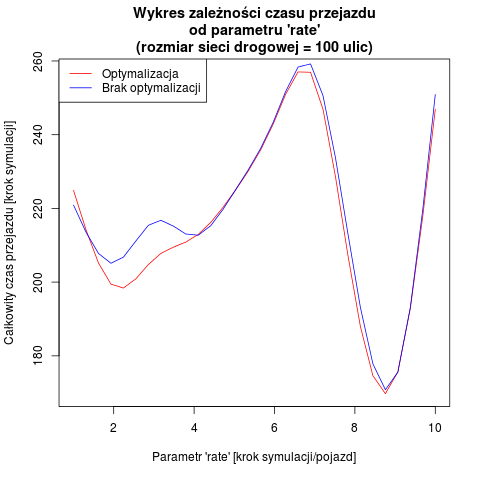
\includegraphics[width=0.7\textwidth]{../images/simulation4}
	\caption{Zależność czasu przejazdu od parametru \textit{rate}.}
\end{figure}


\begin{figure}[H]
	\centering
		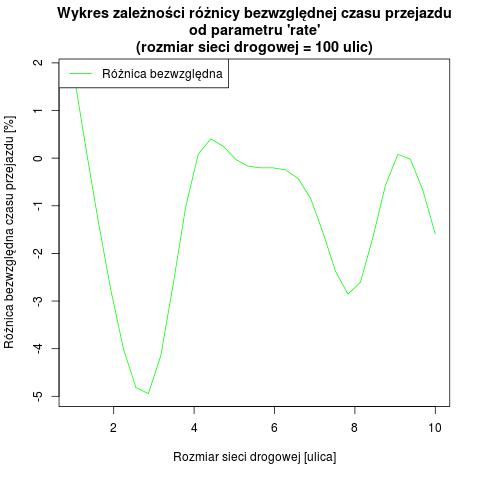
\includegraphics[width=0.7\textwidth]{../images/simulation4_diff}
	\caption{Zależność bezwzględnej różnicy czasów przejazdu od parametru \textit{rate}.}
\end{figure}

\subsubsection{Analiza wyników}

Parametr \textit{rate} określał częstotliwość pojawiania się nowych pojazdów w sieci drogowej, a co za tym idzie wpływał na natężenie ruchu drogowego w sieci. Uzyskane wyniki pozwalają stwierdzić, że dla grafów rozmiaru około stu krawędzi średnie czasy przejazdu są najlepsze dla wartości parametru \textit{rate} wynoszącej około 2 do 3 kroki symulacji na pojazd. Wynika to z trudności znalezienia lepszej trasy dojazdu dla dużego natężenia ruchu drogowego. Z kolei niewielki ruch w sieci drogowej nie powoduje powstawania zatorów i nie wymaga optymalizacji trasy dojazdu.

\subsection{Symulacja 5}

\subsubsection{Opis}

Piąta symulacja była powtórzeniem symulacji czwartej, z tą różnica, że rozmiar sieci drogowej wynosił \textit{1000 ulic}.

\subsubsection{Wyniki}

\begin{table}[H]
\begin{tabular}{ | C{4cm} | C{4cm} | C{4cm} | }
\hline
Parametr 'rate' [krok symulacji/pojazd] & Optymalizacja [krok symulacji] & Brak optymalizacji [krok symulacji] \\ \hline
1 & 578 & 582.1 \\ \hline
2 & 434.1 & 434.9 \\ \hline
3 & 519.6 & 525.4 \\ \hline
4 & 560.3 & 572.9 \\ \hline
5 & 468.1 & 471.1 \\ \hline
6 & 594.4 & 594.4 \\ \hline
7 & 540.8 & 543.9 \\ \hline
8 & 526.3 & 530.1 \\ \hline
9 & 522.7 & 522.7 \\ \hline
10 & 553.6 & 553.6 \\ \hline
\hline
\end{tabular}
\caption{Zależność czasu przejazdu od parametru \textit{rate}.}
\end{table}


\begin{figure}[H]
	\centering
		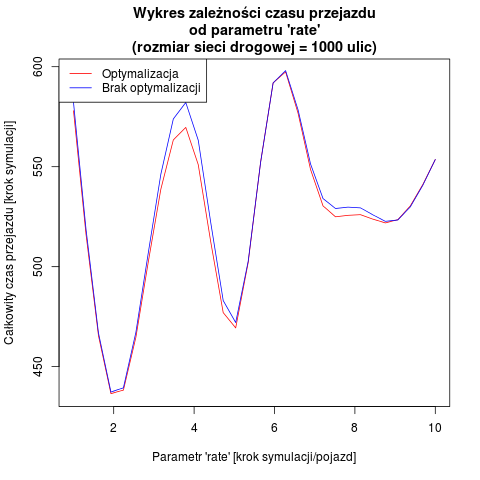
\includegraphics[width=0.7\textwidth]{../images/simulation5}
	\caption{Zależność czasu przejazdu od parametru \textit{rate}.}
\end{figure}

\begin{figure}[H]
	\centering
		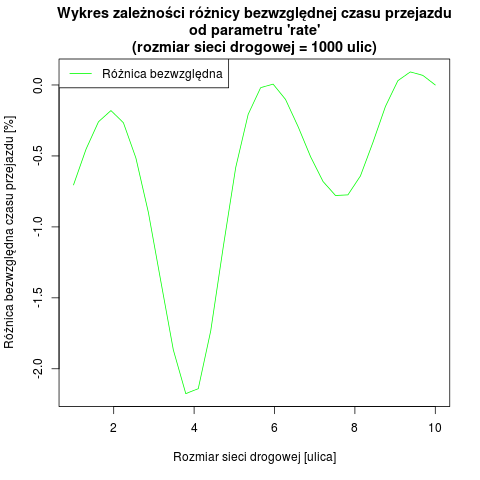
\includegraphics[width=0.7\textwidth]{../images/simulation5_diff}
	\caption{Zależność bezwzględnej różnicy czasów przejazdu od parametru \textit{rate}.}
\end{figure}

\subsubsection{Analiza wyników}

Symulacja piąta podobnie jak symulacja czwarta sprawdzała wpływ parametru \textit{rate} na sumaryczny czas podróży. Wyniki otrzymane w tej symulacji potwierdzają rezultaty poprzedniej symulacji. Ponownie okazuje się, że próba optymalizacji trasy w sposób dynamiczny najkorzystniej wpływa na czas przejazdu dla średniego natężenia ruchu drogowego i daje poprawę rzędu trzech procent.

\subsection{Symulacja 6}

\subsubsection{Opis}

Szósta symulacja miała na celu zbadanie wpływu długości ulic, a co za tym idzie struktury sieci drogowej, na czas podróży. Rozmiar sieci drogowej wynosił \textit{100 ulic}, parametr \textit{alpha 0.05}, a częstotliwość pojawiania się samochodów w sieci drogowej \textit{2 kroki symulacji/pojazd}.

\subsubsection{Wyniki}

\begin{table}[H]
\begin{tabular}{ | C{4cm} | C{4cm} | C{4cm} | }
\hline
Maksymalna długość ulicy [m]& Optymalizacja [krok symulacji] & Brak optymalizacji [krok symulacji] \\ \hline
200 & 152.1 & 154.7 \\ \hline
300 & 241.1 & 243.2 \\ \hline
400 & 188.2 & 195.1 \\ \hline
500 & 299.9 & 306.2 \\ \hline
700 & 245.2 & 245.2 \\ \hline
1000 & 390 & 390.6 \\ \hline
1200 & 368 & 368 \\ \hline
1500 & 669.7 & 670.7 \\ \hline
1700 & 698.7 & 698.8 \\ \hline
2000 & 844.5 & 845.4 \\ \hline
\hline
\end{tabular}
\caption{Zależność czasu przejazdu od maksymalnej długości ulicy.}
\end{table}


\begin{figure}[H]
	\centering
		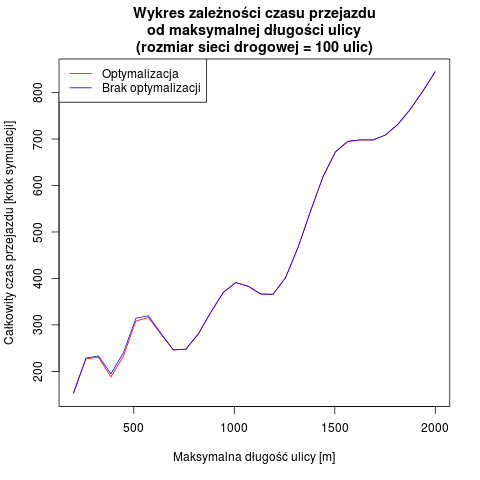
\includegraphics[width=0.7\textwidth]{../images/simulation6}
	\caption{Zależność czasu przejazdu od maksymalnej długości ulicy.}
\end{figure}

\begin{figure}[H]
	\centering
		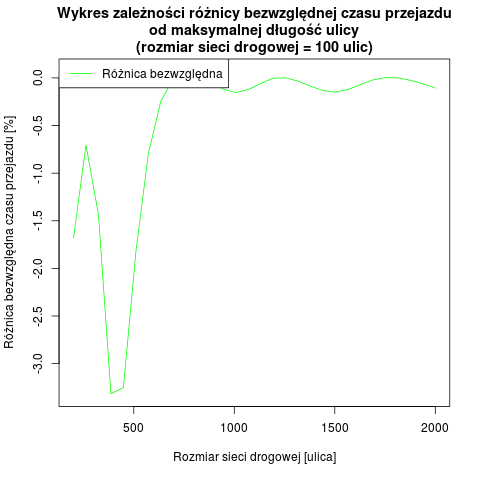
\includegraphics[width=0.7\textwidth]{../images/simulation6_diff}
	\caption{Zależność bezwzględnej różnicy czasów przejazdu od maksymalnej długości ulicy.}
\end{figure}

\subsubsection{Analiza wyników}

Analiza otrzymanych wyników pozwala stwierdzić, że optymalizacja trasy w trybie online wpływa korzystnie na średnie czasy przejazdu. Najlepsze rezultaty dla grafów wielkości około stu krawędzi są uzyskiwane dla stosunkowo krótkich ulic rzędu 300 metrów. Wynika to z faktu, że dla sieci drogowych o zwartej strukturze prawdopodobieństwo powstawania zatorów jest znaczące, a co za tym idzie próby optymalizacji trasy dają korzystniejsze rezultaty.

\subsection{Symulacja 7}

\subsubsection{Opis}

Siódma symulacja była powtórzeniem symulacji szóstej, z tą różnica, że rozmiar sieci drogowej wynosił \textit{1000 ulic}.

\subsubsection{Wyniki}

\begin{table}[H]
\begin{tabular}{ | C{4cm} | C{4cm} | C{4cm} | }
\hline
Maksymalna długość ulicy [m]& Optymalizacja [krok symulacji] & Brak optymalizacji [krok symulacji] \\ \hline
200 & 348.6 & 347.5 \\ \hline
300 & 392.3 & 391.7 \\ \hline
400 & 402.6 & 404.6 \\ \hline
500 & 513.2 & 512.5 \\ \hline
700 & 666.6 & 674.3 \\ \hline
1000 & 800.1 & 815.4 \\ \hline
1200 & 1080.1 & 1095.6 \\ \hline
1500 & 1030.5 & 1029.2 \\ \hline
1700 & 1369.9 & 1394.3 \\ \hline
2000 & 1352.4 & 1369.8 \\ \hline
\hline
\end{tabular}
\caption{Zależność czasu przejazdu od maksymalnej długości ulicy.}
\end{table}


\begin{figure}[H]
	\centering
		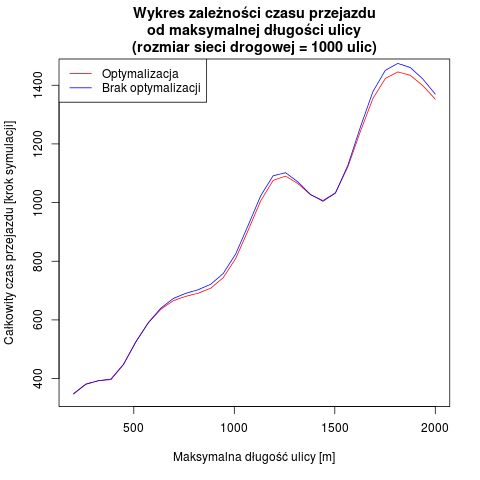
\includegraphics[width=0.7\textwidth]{../images/simulation7}
	\caption{Zależność czasu przejazdu od maksymalnej długości ulicy.}
\end{figure}

\begin{figure}[H]
	\centering
		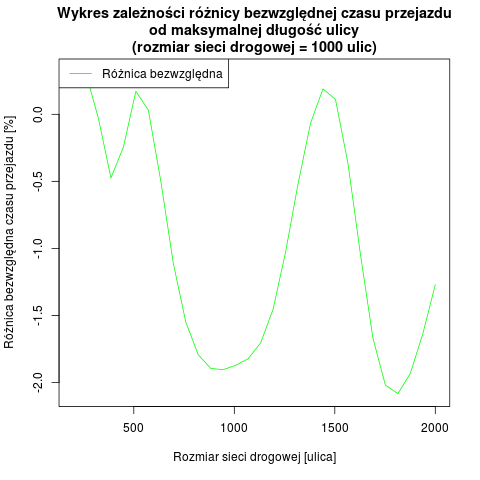
\includegraphics[width=0.7\textwidth]{../images/simulation7_diff}
	\caption{Zależność bezwzględnej różnicy czasów przejazdu od maksymalnej długości ulicy.}
\end{figure}

\subsubsection{Analiza wyników}

Symulacja siódma podobnie jak symulacja szósta sprawdzała wpływ długości ulic, a co za tym idzie także struktury sieci drogowej, na średni czas przejazdu. Wyniki otrzymane w tej symulacji potwierdzają rezultaty poprzedniej symulacji. Ponownie okazuje się, że próba optymalizacji trasy w sposób dynamiczny najkorzystniej wpływa na czas przejazdu dla sieci o stosunkowo zwartej strukturze i daje poprawę rzędu dwóch procent.

\section{Podsumowanie}

Na podstawie serii przeprowadzonych symulacji można stwierdzić, że próby optymalizacji trasy w trybie online dają korzystne wyniki. Średnie czasy przejazdu pojazdu, którego trasa jest dynamicznie zmieniana, są około o dwa do pięciu procent lepsze od czasów przejazdu pojazdu poruszającego się niezmienną trasą. Metoda optymalizacyjna uzyskuje najlepsze rezultaty dla średniego rozmiaru sieci drogowych i średniego natężenia ruchu drogowego.

Należy pamiętać, że przeprowadzone badania miały charakter statystyczny, który wynikał z trudności modelowania nieustannie zmieniającego się ruchu drogowego. Stąd może się okazać, że dla danej sieci i ruchu drogowego metoda optymalizacyjna zakończy się niekorzystnym rezultatem. Jednak dla znakomitej większości przypadków opisana metoda pozwala przebyć zadaną trasę w krótszym czasie, niż gdy nie jest stosowana.

\section{Wykorzystane narzędzia i języki programowania}

W projekcie wykorzystano następujące narzędzia:
\begin{description}
	\item[SUMO] - symulator ruchu drogowego
	\item[Python 2.7] - implementacja modułu symulacyjnego
	\item[R] - graficzna prezentacja wyników
	\item[Visual Paradigm 10.2] - diagramy klas oraz komponentów
	\item[LaTeX] - formatowanie oraz skład dokumentacji
\end{description}

\newpage
\section{Bibliografia}

\begin{enumerate}
	\item \textit{SUMO}
	\url{http://sumo-sim.org/}
	\item \textit{TraCI}
	\url{http://sumo-sim.org/pydoc/traci.html}
	\item \textit{Netgenerate}
	\url{http://sumo-sim.org/userdoc/NETGENERATE.html}
	\item \textit{randomTrips}
	\url{http://sumo-sim.org/userdoc/Tools/Trip.html#randomTrips.py}
	\item \textit{Algorytm Dijkstry}
	\url {http://pl.wikipedia.org/wiki/Algorytm_Dijkstry}
\end{enumerate}

\end{document}
